% !Mode:: "TeX:UTF-8"
% !TEX program = xelatex
\title{Project 5: Solving the FDMs for Two-asset Options}
\author{Iydon Liang}
\date{\today}

\maketitle\tableofcontents\clearpage

\begin{abstract}
    It's clear that how to solve the FDM for one-asset option, either European, American or Path-dependent types. In this report, we discussed the two-asset options case. And gave three methods to determine the price for a two-asset option.
\end{abstract}

\section{Two-asset Option}
\[
    \dd S_i(t) = S_i(t)\alpha_i\dd t + S_i(t)\sigma_i\dd W_i(t)
\]
where $\dd W_i(t)$ $(i=1,\ldots,n)$ are standard Brownian motion which satisfy
\[
    \begin{aligned}
        \EE(\dd W_i) &= 0 \\
        \var(\dd W_i) &= \dd t \\
        \cov(\dd W_i, \dd W_j) &= \delta_{ij} p_{ij} \dd t.
    \end{aligned}
\]

\subsection{Pricing by Monte Carlo Method}
We know that price of the two stocks follows a bi-variate log-normal distribution. And we can generate it from a bi-variate normal distribution with $\mu=0$ and
\[
    \Sigma = \begin{pmatrix}
        1 & \rho \\
        \rho & 1
    \end{pmatrix}.
\]
Then we can sample $(S_1(T), S_2(T))$ from the distribution, and pricing by Monte Carlo method is possible by so.



\section{FDMs for Two-asset Option}
\[
    \frac{\partial V}{\partial t} + rS_1\frac{\partial V}{\partial S_1} + \frac{1}{2}\sigma_1^2S_1^2\frac{\partial^2 V}{\partial S_1^2} + rS_2\frac{\partial V}{\partial S_2} + \frac{1}{2}\sigma_2^2S_2^2\frac{\partial^2 V}{\partial S_2^2} - rV = 0
\]

\subsection{Approximate the Differential Quotients}
Suppose $f(i, j, k) = V(S_1=i\Delta S, S_2=j\Delta S, t=k\Delta k)$,
\[
    \begin{aligned}
        f_t &\approx \frac{f(i, j, k+1) - f(i, j, k)}{\Delta t} \\
        f_{S_1} &\approx \frac{f(i+1, j, k) - f(i-1, j, k)}{2\Delta t} \\
        f_{S_1S_2} &\approx \frac{f(i+1, j, k) - 2f(i, j, k) + f(i-1, j, k)}{\Delta^2S} \\
        f_{S_2} &\approx \frac{f(i, j+1, k) - f(i, j-1, k)}{2\Delta t} \\
        f_{S_1S_2} &\approx \frac{f(i, j+1, k) - 2f(i, j, k) + f(i, j-1, k)}{\Delta^2S}
    \end{aligned}
\]


\subsection{Recursion Form}
Substitute the approximations in to the BS equation, and put $f(\cdot, \cdot, k+1)$ to the left side, put $f(\cdot, \cdot, k)$ to the right hand side. Then we get
\[
    \begin{aligned}
        f(i, j, k+1) =& \quad\alpha_i f(i-1, j, k) \\
        &+ \beta_i f(i+1, j, k) \\
        &+ \gamma_j f(i, j-1, k) \\
        &+ \theta_j f(i, j+1, k) \\
        &+ \lambda_{1i} f(i, j, k) \\
        &+ \lambda_{2j} f(i, j, k)
    \end{aligned}
\]

Here we divide the coefficient of $f(i, j, k)$ into two parts for the convenience of following steps.
\[
    \begin{aligned}
        \alpha_i &= \frac{1}{2}\Delta t(ri-\sigma_1^2i^2) \\
        \beta_i &= -\frac{1}{2}\Delta t(ri+\sigma_1^2i^2) \\
        \gamma_j &= \frac{1}{2}\Delta t(rj-\sigma_2^2j^2) \\
        \theta_j &= -\frac{1}{2}\Delta t(ri-\sigma_2^2j^2) \\
        \lambda_{1i} &= \frac{1}{2} + \Delta t(\frac{1}{2}r+\sigma_1^2i^2) \\
        \lambda_{2j} &= \frac{1}{2} + \Delta t(\frac{1}{2}r+\sigma_2^2j^2) \\
    \end{aligned}
\]


\subsection{Matrix Form}
The relationship can be written as a matrix equation
\[
    AX + XB = C
\]
where matrix $C(i, j) = f(i, j, k+1)$, $X(i, j) = f(i, j, k)$

\begin{figure}[H]
    \centering
    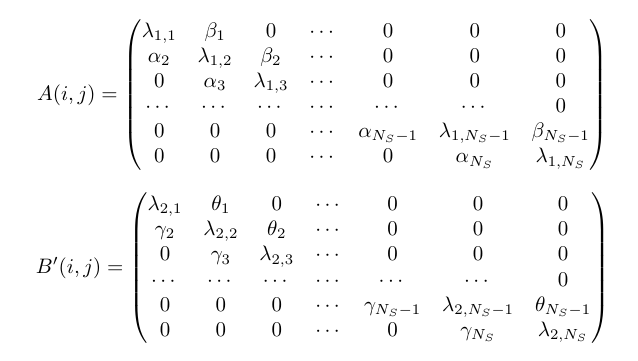
\includegraphics[width=.7\textwidth]{figures/2019-12-25-matrix-form.png}
\end{figure}


\subsection{Solve the Matrix Equation}
Matrix equation of the form $AX + XB = C$ is called \textbf{Sylvester equation}. The equation has a unique solution when the eigenvalues of $A$ and $−B$ are distinct. In \texttt{MATLAB}, there is a function \textbf{sylvester(A,B,C)}, which can solve the Sylvester equation.
